\section{Подходы к моделированию кровотока}
\subsection{Детальное моделирование}
Моделировать кровь можно как жидкость со взвешенными в ней клетками крови, которые могут рассматриваться, как совокупность частиц и сил,
действующих между ними. Эритроциты гораздо крупнее остальных клеток крови и они составляют большую часть её объёма, соответственно они 
и будут определять механические свойства крови. Плазма крови -- раствор крупных молекул, но при масштабах движения и при скоростях
сдвига, обычно встречающихся в кровеносных сосудах, ее можно считать однородной ньютоновской жидкостью  и описывать уравнениями
Новье-Стокса. То есть нам нужно учитывать взаимодействие частиц с жидкостью и друг с другом. Такую задачу удобно решать методом 
диссипативной динамики частиц.

Диссипативная динамика частиц -- это метод, в котором каждая частица описывает небольшой объем моделируемой среды, 
а не отдельную молекулу. Их взаимодействие определяется консервативными $F^C_{ij}$ (не зависящими от траектории), диссипативными 
$F^D_{ij}$ (силы, при действии которых полная механическая энергия  системы убывает, переходя в другие, не механические формы энергии) 
и случайными силами $F^R_{ij}$, действующими между двумя частицами:
\begin{align*}
  &\vec{F^C_{ij}}=F^C_{ij}(r_{ij})\vec{\hat{r}{_{ij}}},\\[10pt]
  &\vec{F^D_{ij}}=-\gamma \omega^D(r_{ij}) (\vec{v_{ij}} \cdot \vec{\hat{r}{_{ij}}})\vec{\hat{r}{_{ij}}},\\[10pt]
  &\vec{F^R_{ij}}=\sigma \omega^R(r_{ij}) \dfrac{\varepsilon_{ij}}{\sqrt{\bigtriangleup t}} \vec{\hat{r}{_{ij}}},
\end{align*}
где $\vec{r_{i}}$— радиус-вектор i-ой частицы, $\vec{r_{ij}}=\vec{r_{j}} - \vec{r_{j}}$,
$r_{ij}=|\vec{r_{ij}}|$,
$\vec{\hat{r}{_{ij}}}=\vec{r_{ij}}/{r_{ij}}$,
$\vec{v_{ij}}=\vec{v_{j} - \vec{v_{j}}}$ -- разница между скоростями двух частиц, $\bigtriangleup t$ -- шаг по времени, 
$\gamma, \sigma$ -- это  коэффициенты, определяющие силу диссипативной и случайной силы соответственно, а $\omega^R,\omega^D$ -- весовые функции,
${\varepsilon_{ij}={\varepsilon_{ji}}}$ -- нормально распределенная случайная величина с нулевым средним и единичной дисперсией.

Мембрана эритроцита практически несжимаема и устойчива к изменению площади поверхности деформации сдвига в плоскости. 
Она может быть смоделирована как двумерная сеть частиц соединенных пружинами, смоделированными по закону Гука 
и образующих неправильный многогранник с треугольными гранями Рис.~\ref{elasticity scheme}.

\begin{figure}[h]
\centering
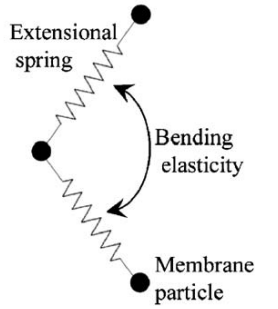
\includegraphics[width=0.2\linewidth]{mol3.png}
\caption{ Схема упругости при растяжении и изгибе между частицами в мембране~\cite{hosseini:2009}.}
\label{elasticity scheme}
\end{figure}

Для её описания используется четыре силы.
Первая сила возникает, когда стороны треугольников меняют свою длину.
$$
\vec {F_I}=k_I\left(1- \frac{l}{l_0}\right)\vec\tau,
$$
где $l$ -- длина ребра, $l_0$ -- равновесная длина, $k_I$ -- коэффициент жёсткости, $\vec {\tau}$ -- единичный вектор, 
направленный от одной вершины к другой.

К каждому узлу сходится несколько сторон, и каждая из них вносит свой вклад в общую силу F. 
Вторая сила определяется сжатием или расширением мембраны 
$$
{p_s}=k_s\left(1- \frac{s}{s_0}\right),
$$
где $s$ -- площадь треугольника, $s_0$ -- площадь равновесного треугольника, $k_s$ -- коэффициент расширения площади.

Третья сила пропорциональна изменению объема многогранника и прикладывается к вершинам треугольников в направлении, нормальном к поверхности 
$$
\vec{F_v}=k_v\left(1- \frac{v}{v_0}\right) s \vec{n},
$$
где $v$ -- объем многогранника, $v_0$ -- равновесный объем, $k_v$ -- коэффициент, $s$ -- площадь
треугольного элемента, а $n$ -- единичный нормальный вектор к этому треугольнику.

Четвёртая сила выражается через изгибающий момент~\cite{hosseini:2009} 
$$
 \vec{M_i}=k_M \tan\left(\frac{\theta}{2}\right)l \vec{\tau_i},
$$
где $\theta$ -- угол между соседними треугольными элементами, 
$k_m$ -- коэффициент жесткости, $\vec{\tau_i}$ -- единичный вектор, сонаправленный с общим краем двух треугольников 
и $l$ -- длина этой стороны.

Аналогичным образом могут быть смоделированы и другие клетки крови. Например, в отличие от эритроцитов, лейкоциты содержат ядро. 
Из-за этого они менее деформируемы, а их форма близка к сфере. Это влияет на их поведение в потоке крови.

Для определения параметров эритроцитов прибегают к методам численного моделирования~\cite{bessonov:2014}.

Фактически, можно легко указать на несколько недостатков данной модели. Например, рассмотрение всей клетки как однородной решетки 
делает невозможным учет любой органеллы в цитоплазме. Кроме того, эффективная упругость решетки зависит не только от 
пружинной постоянной, но и от конкретной формы, размера и топологии решетки. Это затрудняет сравнение между различными моделями 
и экспериментами. Более того, параметры модели на уровне частиц  модели не были систематически связаны с физиологическими измерениями; 
они должны принимать нереальные значения, чтобы предсказание было количественно сопоставимо с реальностью 


\subsection{Моделирование крови как вязкой жидкости}
Жидкость может считаться ньютоновской, если она удовлетворяет закону вязкости Ньютона, 
т.е. напряжение сдвига пропорционально скорости сдвига, а вязкость является константой пропорциональности, 
поэтому плазму крови, состоящую в основном из воды, можно считать ньютоновской. Однако у крови более сложные механические свойства. 
И мы предполагаем, что все макроскопические масштабы длины и времени достаточно велики по сравнению с масштабами длины и времени 
на уровне отдельного эритроцита. Таким образом, для упрощения построения модели и дальнейшей работы с ней можно рассматривать 
взвешенные клетки в плазме, как вязкую несжимаемую, неньютоновскую жидкость.

Такие методы применяется в тех сосудах, где клетки достаточно малы и многочисленны, чтобы их отдельную индивидуальность можно было
игнорировать, а их влияние на движение всей крови описывать усредненным способом. 
Так обстоит дело в крупных артериях (диаметр аорты, например, примерно в 2000 раз больше диаметра эритроцита). 
На практике эти методы применяются в изучении и моделировании сердечного выборса, печеночного кровотока, среднего артериального давления.

\textbf{Вязкость.}
Для начала рассмотрим простейшую конститутивную модель, основанную на предположении, что тензор дополнительных напряжений пропорционален
симметричной части градиента скорости.
$$
\tau=2\mu (\dot{\gamma})D,
$$
где $\tau $ -- тензор дополнительных напряжений, $D=(\nabla u+\nabla u^T)$ -- тензор скорости деформации, 
$\mu (\dot{\gamma})$ -- скорость сдвига.
Зависимость $\mu (\dot{\gamma})$ находят разными способами. Например, в~\cite{walburn:1976}, 
рассматривают зависимость вязкости от гематокрита и белка минус-альбумин: \\
$$
\mu (\dot{\gamma})=K{\gamma}^{n-1}, \qquad  K=C_1 \exp (C_2 H_t).
$$
Полученные таким способом результаты вязкости оказались схожи с результатами, которые были получены в~\cite{kim:2000} при помощи вязкозиметра.\\

\textbf{Вязкоупругость.}
Вязкоупругие жидкости -- это вязкие жидкости, обладающие способностью накапливать и высвобождать энергию. 
Упругая энергия объясняется свойствами мембраны РНК, демонстрирующей релаксацию~\cite{evans:1976} и зависящей от скорости сдвига.\\
Одной из простейших моделей, учитывающих вязкоупругость крови, является модель Максвелла~\cite{thurston:1972}:
$$
\tau+\lambda_1(\delta\tau / \delta t)=2\mu D,
$$  
где $\lambda_1$ -- время релаксации, a $\delta\tau / \delta t$ -- обобщение материальной производной по времени.
При построении данной модели полагают, что время релаксации зависит от скорости сдвига.
В~\cite{thurston:1994} данный метод используют для понимания неньютоновского вязкого характера крови после устойоявшегося поток.\\

\textbf{Предел текучести.}
Предел текучести обычно рассматривается как постоянное материальное свойство жидкости. 
Но зафиксированные пределы текучести имели большой разброс, который, стоит отметить, зависел от множества факторов.
Поэтому предел текучести стоит рассматривать не как константу, а как функцию времени и связанную с тиксотропией, 
как было предложено в~\cite{moller:2006}.
Более популярной моделью предела текучести является модель Кассона.
$$
\begin{aligned}
	&\sqrt{II_\tau} < \tau_Y\longrightarrow D=0 \\
	&\sqrt{II_\tau} \geq \tau_Y\longrightarrow
	\begin{cases}
		D   = \dfrac{1}{2\mu N}\left(1-\dfrac{\sqrt{\tau_Y}}{II_\tau}\right)^2\tau \\[10pt]
		\tau= 2\left(\sqrt{\mu N}+\dfrac{\sqrt{\tau_Y}}{\sqrt[4]{4II_D}}\right)^2
	\end{cases}
\end{aligned}
$$

В нашем случае предел текучести является параметра крови, например, для понимания, как будет вести себя кровь под влиянием какого-либо 
препарата, не станет ли она слишком вязкой или наоборот.
Однако, до сих пор использование предела текучести в качестве параметра моделирования крови остаётся спорным, 
в связи с неточностями его определения.

\subsection{Одномерные модели}
Данное семейство методов основано на осреднении трёхмерных характеристик течения по поперечному сечению и сведении
трёхмерной дифференциальной задади о движении крови по сосуду к одномерной.
Для описании сети кровеносных сосудов используются условия сохранения расхода и полного давления в точках бифуркации.

Привлекательность oдномерныx моделeй кровотока основана на разумных вычислительных затратах. 
Основные приложениями этих моделей являются транспорт газов крови и лекарств в организме, перераспределение кровотока при внешних 
или внутренних воздействиях, перераспределение кровотока в результате внутрисосудистых операций. Основными недостатками данных моделей 
являются сложность численных схем, высокая стоимость вычислений и спекулятивные граничные условия. 
Вычислительная область -- это сосудистая одномерная сеть человека или ее части. 
Сеть может быть создана на основе общих анатомических данных, таких как справочник анатомических карт~\cite{bunicheva:2013}, 
анатомические 3D модели или данные конкретного пациента.

Обозначим через $t$ -- время, через $x$ -- координату вдоль сосуда, через $A(t, x)$ -- площадь поперечного сечения сосуда, 
$u(t, x)$ и $p$ -- усредненную по сечению линейную скорость и трансмуральное давление крови. Баланс массы и импульса в переменных 
$(A, u, p)$ соответствует уравнениям
\begin{align}
    \label{eq:mass-balance}
    \varphi=&\frac{\partial A}{\partial t}+\frac{\partial Au}{\partial x},\\
    \label{eq:momentum-balance}
    \psi=&\frac{\partial u}{\partial t}+ \frac{\partial u^2/2+p/\rho}{\partial x}
\end{align}
Правые части уравнений (масса источника или поглотителя на единицу длины, ускорение в результате внешних воздействий) зависят от моделируемого процесса. 

Неизвестными в этих уравнениях являются осреднённые значения $u$, $p$ и $A$.
В одномерных моделях кровотока традиционное описание упругих свойств стенки сосуда обеспечивается зависимостью давления от площади 
поперечного сечения $p(A)$. Прямой подход к получению отношения $p(A)$ включает в себя точное одновременное измерение в естественных 
условиях давления и площади в разные моменты времени. Но такой метод не всегда удобен в реальности.

Качественный анализ физических экспериментов подтверждает, что функция $p(A)$ должна быть монотонной S-подобной кривой. 
Такая кривая удовлетворительно описывает  состояния как круглого, так и эллиптического сечения. 
На практике S-подобная зависимость давления от площади часто аппроксимируется аналитической функцией. 

\begin{figure}[h]
\centering
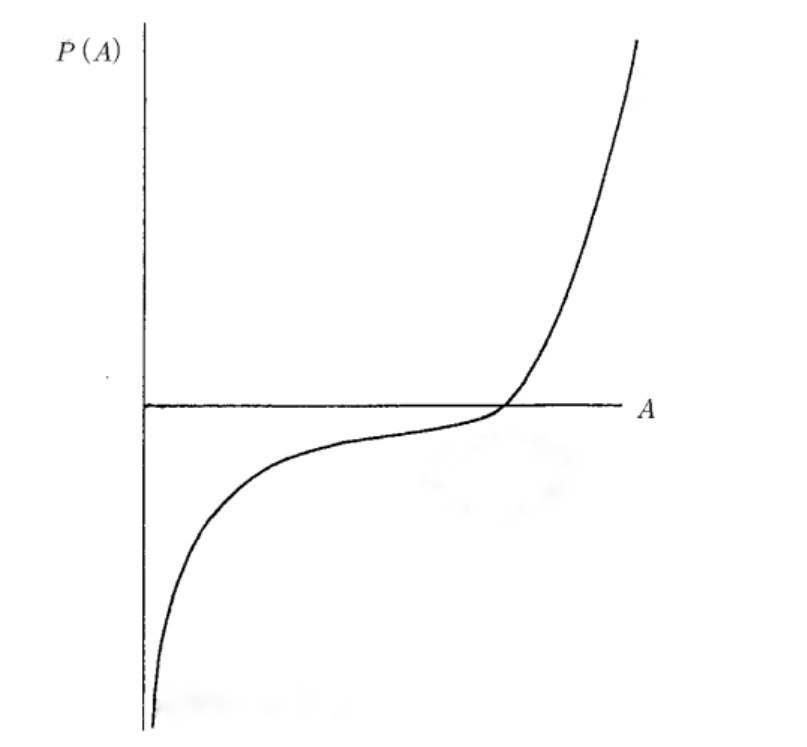
\includegraphics[width=0.3\linewidth]{IMG_20230309_021324_943-01.jpeg}
\caption{ График зависимости $p(A)$~\cite{pedly:1998}.}
\label{fig:mpr}
\end{figure}
Другие обобщения модели эластичной стенки сосуда являются модели вязкоупругой стенки. В таких моделях зависимость выражается в виде
$
p(A)=F(A,\partial {A} / \partial {t},\partial^2{A} / \partial {t^2},\partial^2{A} / \partial {x^2})
$.

%Эта модель была использована в~\cite{bunicheva:2004} для моделирования воздействия гравитационной перегрузки на системное кровообращение. 

Правильные упругие свойства артерий и вен могут быть описаны следующей функцией~\cite{holodov:2001}:
\begin{equation}
    \label{eq:elastic-propeties}
    p(A)=\rho c^2_0 f(a/a_0), 
    \quad
    f(k)=\begin{cases}
    \exp(k-1)-1, &k>1 \\ \ln(k), &k \leq 1
    \end{cases}
\end{equation}

В случае рассмотрения сети сосудов уравнения сохранения массы и импульса(\ref{eq:mass-conserv}),(\ref{eq:mom-conserv}). 
записываются для каждого k-го сосуда. C учётом упругих свойств сосудов (\ref{eq:elastic-propeties}) получим  
\begin{align}
    \label{eq:mass-conserv}
    \frac{\partial A_k}{ \partial t} + \frac{\partial(u_kA_k)}{\partial x}&=\varphi _k(t,x,S_k,u_k,r_i),\\
    \label{eq:mom-conserv}
    \frac{\partial u_k}{\partial t} + \frac{\partial(u_k^2/2+p_k/\rho_k)}{\partial x}&= \psi_k(t,x,S_k,u_k,r_i),\\
    \label{eq:t-pressure}
    p_k(t,x)-p_*(t,x)&=\rho_k c^2_{k0}f_k(S_k(t,x)),
\end{align}
где $t$ -- время, $x$ -- расстояние вдоль сосуда, $\rho$=const -- плотность, $c_{k0}(t,x)$ -- скорость распространения малых возмущений,
  $p_k(t,x)$ -- давление внутри сосуда (от атмосферного) $p_*(t,x)$ -- избыточное давление в тканях, окружающих сосуд, 
  $A_ku_k=Q(t,x)$ -- объёмный расход, $\varphi_k(t,x,S_k,u_k,r_i)$ -- источник/утечка массы, $\psi_k(t,x,S_k,u_k,r_i)$ -- внечние силы (гравитация, трение и т.~д.),
  $k=1,2,\ldots$ -- индекс сосуда.
\\ 

{\bf Граничные условия.}
Для одномерных моделей кровотока необходимы граничные условия на стыках сосудов, входах и выходах в сети сосудов.
Для всех сосудов граничные условия должны включать условия совместимости по характеристикам системы гиперболических уравнений (\ref{eq:mass-balance}), (\ref{eq:momentum-balance})~\cite{Xiu:2007}.
В каждой конечной точке сосуда требуется только одно дополнительное условие совместимости.
Вторым условным граничным условием на стыке N сосудов является сохранение массы:
\begin{equation}
    \label{eq:conserv-mass}
    \sum_{k=k_1,k_2,...,k_N} \varepsilon_k A_k(t,x_k)u_k(t,x_k)=0,
\end{equation}
где {$k_1,...,k_N$} -- индексы сосудов, $\varepsilon_k=1, x_k=0$ -- для входящих сосудов,
$\varepsilon_k=1, x_k=L_k$ -- для выходящих сосудов.
Также используется $N$ интегральных условий сохранения Бернулли выражающих непрерывность полного давления $P^l$:
\begin{equation}
    \label{eq:bernulli}
    \frac{\rho u^2_k}{2}+{p_k(A_k)}=P^l.
\end{equation}
Иногда для моделирования сопротивления потоку в местах стыка используют условия перепада давлений
с учётом сопротивления
\begin{equation}
    \label{eq:p-pressure}
    p_k\left(A_k\left(t,x_k\right)\right)-p^l(t)=\varepsilon_k R^l_k A_k(t,x_k)u_k(t,x_k),
\end{equation}
которое выражается через коэффициент $R^l_k$. Здесь $p^l$ -- давление в точке бифуркации \cite{bessonov:2014}.


Выходы сети артерий и входы сети вен должны быть связаны с множеством мелких неучтенных сосудов, относящихся к микрососудистым регионам.
 Поток в таких сосудах не может быть описан одномерными моделями течения (\ref{eq:mass-balance})-(\ref{eq:mass-conserv})
 из-за большого количества сосудов, сложной структуры микрососудистых сетей и неньютоновской реологии крови.

Более простой подход заключается в том, чтобы объединить артерий и вены в точки соединения,
где выполняются (\ref{eq:conserv-mass}),(\ref{eq:p-pressure}). Коэффициенты сопротивления $ R^l_k$ оцениваются  по известному перепаду
давления между артериями и венами. Чем больше сосудистая сеть, тем меньше сосудов объединяются, тем выше точность метода.
Более подходящие граничные условия оттока: отдельные участки мелких артерий и микроциркуляции моделируются как структурированные деревья,
чей импеданс корней может быть оценен из линеаризации управляющих уравнений.

Многие авторы~\cite{alastruey:2008} выполняют сопряжение во временной области 1D моделей кровотока с электрическими цепями
(единичными параметрами) 0D моделей. 0D модели обеспечивают корректные граничные условия для глобальных моделей кровотока.
\\
\subsection{Вывод}
Были рассмотрены три семейства методов моделирования течения крови в организме.
Методы детального моделирования рассматривают течение мелкодисперсной суспензии
и подробно учитывают эффекты связанные с влияние клеток крови на поток.
Из-за большой вычислительной сложности эти методы можно применять
только для расчётов очень небольших участков сосудов.
Методы моделирования, основанные на решении задачи о течении вязкой жидкости,
пренебрегают прямым учётом наличия клеток в потоке, а связанные с этим эффекты
учитываются через модификацию значения вязкости потока.
Такие методы менее требовательны к вычислительной мощности и имеют более широкое применение. С их помощью могут быть решены
задачи о течении в отдельном сосуде или даже нескольких связанных сосудах.
Методы одномерного моделирования решают задачу в одномерной осреднённой постановке и могут быть
применены для расчёты всей сердечно-сосудистой системы в целом.
